\documentclass[tikz,border=10pt]{standalone}
\begin{document}
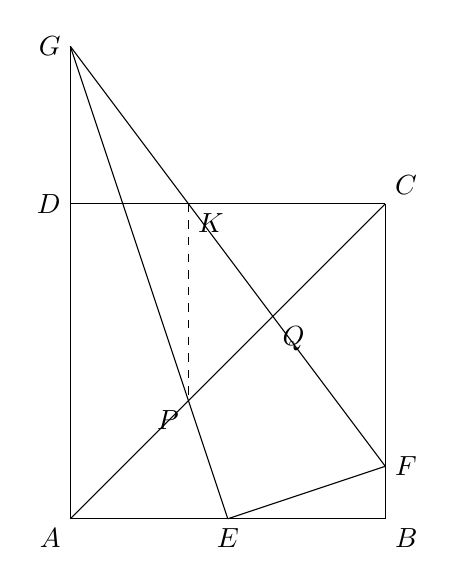
\begin{tikzpicture}
    \coordinate (A) at (0,0);
    \coordinate (B) at (4,0);
    \coordinate (C) at (4,4);
    \coordinate (D) at (0,4);
    \coordinate (G) at (0,6);
    \coordinate (E) at (2,0);
    \coordinate (F) at (4,2/3);
    \coordinate (P) at (1.5,1.5);
    \coordinate (K) at (1.5,4);
    \coordinate (Q) at (18/7,18/7);

    \draw (A) -- (B);
    \draw (B) -- (C);
    \draw (C) -- (D);
    \draw (A) -- (G);
    \draw (A) -- (C);
    \draw (G) -- (E);
    \draw (G) -- (F);
    \draw (E) -- (F);
    \draw[dashed] (K) -- (P);

    \node[below left] at (A) {$A$};
    \node[below right] at (B) {$B$};
    \node[above right] at (C) {$C$};
    \node[left] at (D) {$D$};
    \node[below] at (E) {$E$};
    \node[right] at (F) {$F$};
    \node[left] at (G) {$G$};
    \node[below left] at (P) {$P$};
    \node[below right] at (K) {$K$};
    \node[below right] at (Q) {$Q$};
\end{tikzpicture}
\end{document}
